\begin{figure*}\centering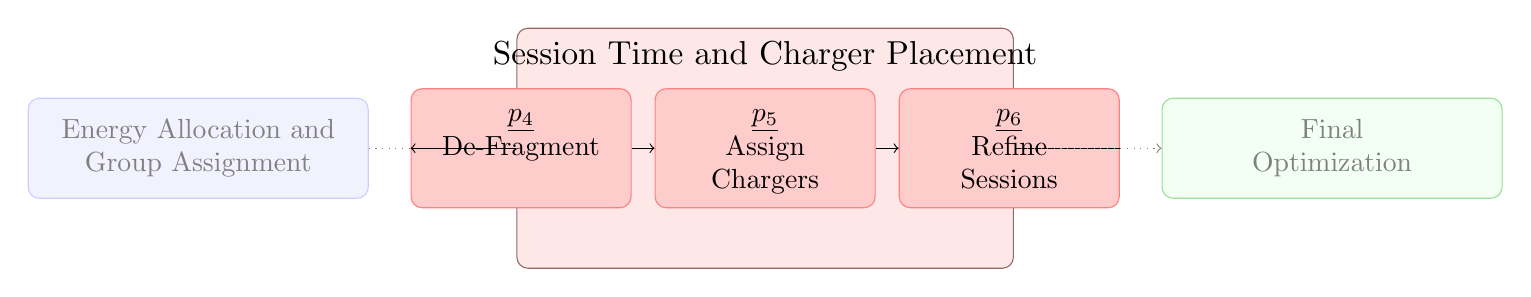
\begin{tikzpicture}
\node[rectangle, draw=gray!80!red, fill=gray!10!red!10, minimum width=\textwidth*0.52, minimum height=1.2in, rounded corners, label={[label distance=-0.67cm]above:\scalebox{1.2}{Session Time and Charger Placement}}](outline) at (0,0){};
	\node[rectangle, draw=red!50, fill=red!20, minimum width=1.1in, minimum height=0.5in, rounded corners](problem1) at (-3.1,0) {\begin{tabular}{c} \underline{$p_4$} \\ De-Fragment \\  \\\end{tabular}}; 
	\node[rectangle, draw=red!50, fill=red!20, minimum width=1.1in, minimum height=0.5in, rounded corners](problem2) at (0,0) {\begin{tabular}{c}\underline{$p_5$} \\ Assign\\ Chargers\end{tabular}}; 
	\node[rectangle, draw=red!50, fill=red!20, minimum width=1.1in, minimum height=0.5in, rounded corners](problem3) at (3.1,0) {\begin{tabular}{c}\underline{$p_6$} \\ Refine\\ Sessions\end{tabular}}; 
	\node[rectangle, draw=blue!20, fill=blue!5, text=black!50, minimum width=1.7in, minimum height=0.5in, rounded corners](problem0) at (-7.2,0){\begin{tabular}{c}Energy Allocation and\\ Group Assignment\end{tabular}};
	\node[rectangle, draw=green!70!black!40, fill=green!5, text=black!50, minimum width=1.7in, minimum height=0.5in, rounded corners](problem4) at (7.2,0){\begin{tabular}{c}Final \\ Optimization\end{tabular}};
	\draw[draw=black!50, dotted] (problem0.east) -- (outline.west);
	\draw[->] (outline.west) -- (problem1.west);
	\draw (problem3.east) -- (outline.east);
	\draw[->, draw=black!50, dotted] (outline.east) -- (problem4.west);
	\draw[->, draw=black] (problem1.east) -- (problem2.west);
	\draw[->, draw=black] (problem2.east) -- (problem3.west);
\end{tikzpicture}\caption{Processing chain for each group} \label{fig:set2Chain}\end{figure*}

